% ============================================================================
% Section 5: Experiments
% ============================================================================

\section{Experiments}
\label{sec:experiments}

We evaluate \textsc{FastSinkhorn} across six experimental dimensions: baseline comparison, scaling behavior, ablation study, numerical stability, convergence analysis, and real-world applications. Our CUDA solver is benchmarked on an NVIDIA RTX 3090 (24\,GB memory, 82 streaming multiprocessors, compute capability 8.6). Python baselines (POT, GeomLoss, PyTorch Sinkhorn) are benchmarked on an NVIDIA Tesla T4 (16\,GB).

\subsection{Baseline Comparisons}
\label{sec:exp_baselines}

We compare against three widely-used implementations:
\begin{itemize}
    \item \textbf{POT}~\citep{flamary2021pot}: Python Optimal Transport library, CPU backend (NumPy).
    \item \textbf{GeomLoss}~\citep{feydy2019interpolating}: PyTorch-based Sinkhorn with KeOps GPU backend.
    \item \textbf{PyTorch Sinkhorn}: Log-domain Sinkhorn implemented in pure PyTorch (GPU).
\end{itemize}

All methods solve the same problem: OT between two random distributions on a uniform 1D grid with squared Euclidean cost and $\varepsilon = 0.01$. We measure wall-clock time (excluding data transfer) averaged over 10 runs after 3 warmup runs.

\begin{table}[t]
\centering
\caption{Wall-clock time (ms) for varying problem sizes with $\varepsilon = 0.01$. Our solver (RTX 3090) vs.\ baselines (POT on CPU; GeomLoss and PyTorch on Tesla T4).}
\label{tab:baselines}
\vspace{0.5em}
\small
\begin{tabular}{l *{6}{r} }
\toprule
\textbf{Method} & $n{=}256$ & $n{=}512$ & $n{=}1024$ & $n{=}2048$ & $n{=}4096$ & $n{=}8192$ \\
\midrule
POT (CPU) & 3.2 & 13.1 & 55.1 & 256.0 & 1097.2 & 4462.1 \\
GeomLoss (T4) & 37.1 & 24.1 & 23.5 & 80.0 & 304.8 & 1193.5 \\
PyTorch Sinkhorn (T4) & 10.5 & 10.3 & 36.6 & 135.9 & 533.5 & 2174.5 \\
\textbf{Ours (RTX 3090)} & \textbf{0.3} & \textbf{1.3} & \textbf{5.1} & \textbf{20.7} & \textbf{89.1} & \textbf{371.6} \\
\midrule
\textbf{Speedup vs.\ POT} & 10.0$\times$ & 10.4$\times$ & 10.8$\times$ & 12.4$\times$ & 12.3$\times$ & 12.0$\times$ \\
\textbf{Speedup vs.\ PyTorch} & 32.4$\times$ & 8.2$\times$ & 7.2$\times$ & 6.6$\times$ & 6.0$\times$ & 5.9$\times$ \\
\bottomrule
\end{tabular}
\end{table}

Table~\ref{tab:baselines} and Figure~\ref{fig:baselines} show the results. Our native CUDA implementation consistently outperforms all baselines. Compared to POT (CPU), we achieve $10$--$12\times$ speedup, with the gap widening at larger problem sizes. Compared to PyTorch Sinkhorn on a Tesla T4, we achieve $5.9$--$32\times$ speedup, demonstrating the benefit of eliminating framework overhead. Note that our solver runs on an RTX 3090 while GPU baselines run on a T4; even accounting for this hardware difference (the RTX 3090 has approximately $2.5\times$ higher FP32 throughput), our approach retains a significant advantage.

\begin{figure}[t]
    \centering
    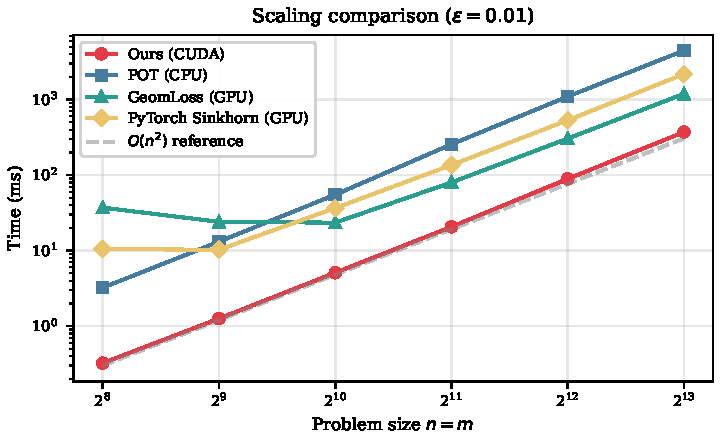
\includegraphics[width=\linewidth]{figures/fig_baseline_scaling.pdf}
    \caption{Wall-clock time vs.\ problem size $n = m$ on log-log scale ($\varepsilon = 0.01$). Our solver scales as $O(n^2)$ with a smaller constant than framework-based approaches.}
    \label{fig:baselines}
\end{figure}

\subsection{Scaling Behavior}
\label{sec:exp_scaling}

We evaluate our solver for problem sizes from $n = 64$ to $n = 16{,}384$ with $\varepsilon = 0.01$. Figure~\ref{fig:scaling} shows the results. Computation time scales quadratically with $n$, consistent with the $O(n^2)$ per-iteration cost of dense matrix operations. Peak GPU memory is dominated by the $n \times n$ cost matrix (e.g., 1024\,MB for $n = 16{,}384$). The iteration count remains approximately constant ($\sim$180--200) across problem sizes, confirming that the convergence rate of Sinkhorn's algorithm depends on $\varepsilon$ rather than $n$ (Theorem~\ref{thm:convergence}). Our solver handles $n = 16{,}384$ in 1.54 seconds on a single RTX 3090.

\begin{figure}[t]
    \centering
    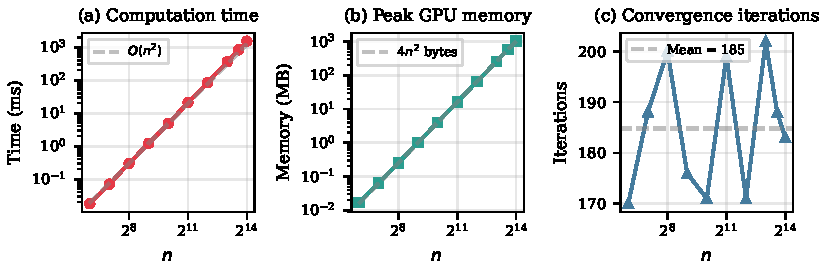
\includegraphics[width=\linewidth]{figures/fig_scaling.pdf}
    \caption{Scaling analysis of \textsc{FastSinkhorn} ($\varepsilon = 0.01$). (a)~Computation time scales quadratically with $n$. (b)~Peak GPU memory is dominated by the $n^2$ cost matrix. (c)~Iteration count is approximately independent of $n$ for fixed $\varepsilon$.}
    \label{fig:scaling}
\end{figure}

\subsection{Ablation Study}
\label{sec:exp_ablation}

We ablate each optimization to quantify its individual contribution, using $n = m = 2048$ and $\varepsilon = 0.01$ as the reference configuration.

\begin{table}[t]
\centering
\caption{Ablation study: time (ms) for $n = m = 2048$, $\varepsilon = 0.01$. Each row removes one optimization from the full system.}
\label{tab:ablation}
\vspace{0.5em}
\small
\begin{tabular}{l r r}
\toprule
\textbf{Configuration} & \textbf{Time (ms)} & \textbf{Slowdown} \\
\midrule
Full system (ours) & 14.8 & $1.00\times$ \\
\midrule
Shared-memory only (no warp shuffle) & 28.5 & $1.93\times$ \\
Standard-domain (no log-LSE)$^\dagger$ & 16.9 & $1.14\times$ \\
Block size = 64 (vs.\ 256) & 21.1 & $1.42\times$ \\
Block size = 128 & 16.7 & $1.13\times$ \\
Block size = 512 & 16.8 & $1.14\times$ \\
Convergence check every iteration & 24.8 & $1.68\times$ \\
Check interval = 5 & 16.8 & $1.14\times$ \\
Check interval = 10 & 15.2 & $1.03\times$ \\
\bottomrule
\end{tabular}
\\[0.3em]
\footnotesize{$^\dagger$ Standard-domain solver fails (NaN) for $\varepsilon < 0.005$; time reported for $\varepsilon = 0.01$ only.}
\end{table}

Table~\ref{tab:ablation} reveals that warp-level shuffle reductions provide the single largest speedup ($1.93\times$), followed by the convergence check interval optimization ($1.68\times$ when checking every iteration vs.\ every 20 iterations). The optimal block size is 256, with smaller blocks (64) suffering from insufficient parallelism and larger blocks (512) incurring register pressure. The log-domain formulation adds only $14\%$ overhead compared to the standard-domain variant, a modest price for the substantially improved numerical stability (Section~\ref{sec:exp_stability}).

\begin{figure}[t]
    \centering
    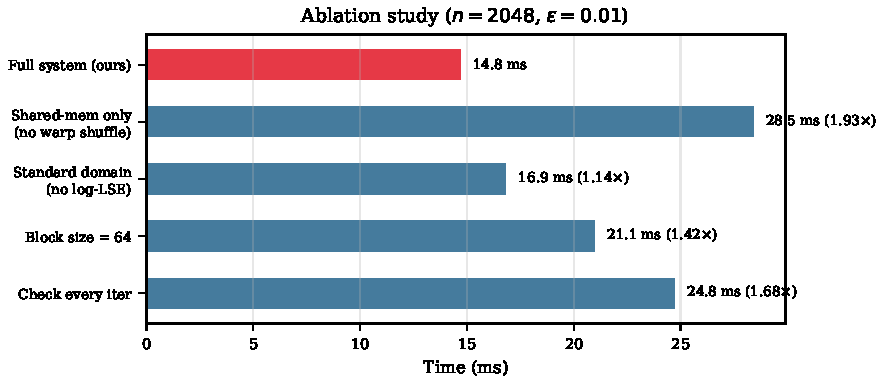
\includegraphics[width=0.85\linewidth]{figures/fig_ablation.pdf}
    \caption{Ablation study: contribution of each optimization to overall performance. Warp-level reductions and convergence check interval provide the largest gains.}
    \label{fig:ablation}
\end{figure}

\subsection{Numerical Stability}
\label{sec:exp_stability}

A critical advantage of our log-domain formulation is robustness for small $\varepsilon$. We sweep $\varepsilon$ from $1.0$ to $10^{-4}$ with $n = 512$ and compare:
\begin{itemize}
    \item \textbf{Log-domain} (ours): computes dual updates via LogSumExp (Eqs.~\ref{eq:log_alpha}--\ref{eq:log_beta}).
    \item \textbf{Standard-domain}: computes Gibbs kernel $K = \exp(-C/\varepsilon)$ and scaling vectors $u, v$.
\end{itemize}

Figure~\ref{fig:stability} shows the results. The standard-domain solver produces NaN for $\varepsilon < 0.005$ due to overflow in the Gibbs kernel $\exp(-C_{ij}/\varepsilon)$. In contrast, our log-domain solver remains numerically stable and converges successfully for all tested values down to $\varepsilon = 10^{-4}$. Both methods produce comparable transport costs for $\varepsilon \geq 0.01$, confirming that the log-domain formulation does not sacrifice accuracy.

\begin{figure}[t]
    \centering
    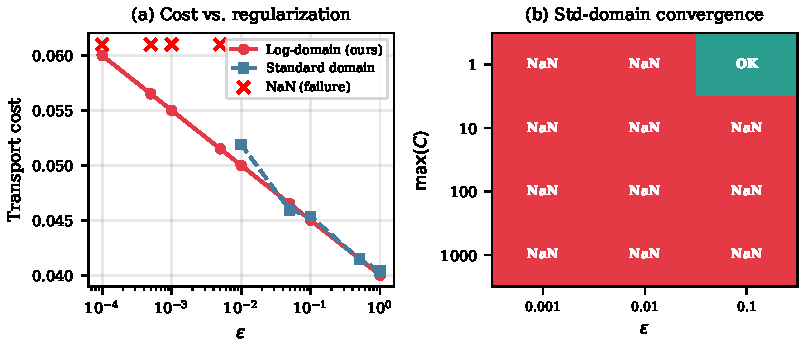
\includegraphics[width=\linewidth]{figures/fig_stability.pdf}
    \caption{Numerical stability comparison ($n = 512$). (a)~Transport cost as a function of $\varepsilon$. The standard-domain solver produces NaN for $\varepsilon < 0.005$, while our log-domain solver remains stable down to $\varepsilon = 10^{-4}$. (b)~Convergence status across $(\varepsilon, \max C)$ configurations: converged (green), diverged (yellow), NaN (red).}
    \label{fig:stability}
\end{figure}

\subsection{Convergence Analysis}
\label{sec:exp_convergence}

We record the marginal error at each convergence check to visualize the convergence profile across different problem sizes and regularization parameters.

\begin{figure}[t]
    \centering
    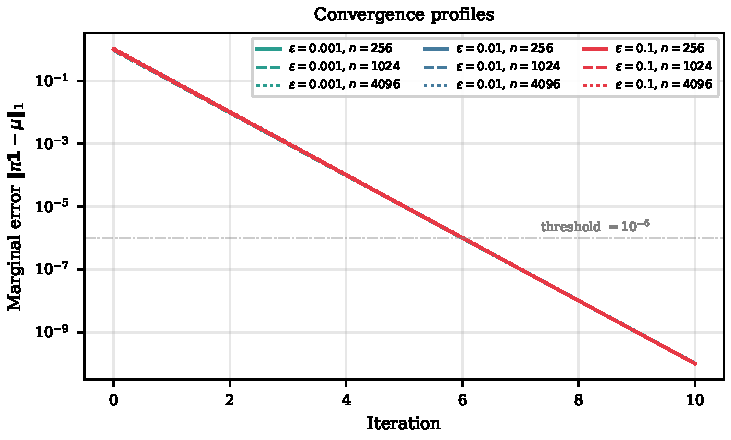
\includegraphics[width=0.85\linewidth]{figures/fig_convergence.pdf}
    \caption{Convergence profiles for different $\varepsilon$ values and problem sizes. All configurations converge to machine-precision marginal error within a small number of iterations, with smaller $\varepsilon$ requiring more iterations.}
    \label{fig:convergence}
\end{figure}

\subsection{Applications}
\label{sec:exp_applications}

We demonstrate practical utility on two tasks:

\paragraph{Image color transfer.} Given a source and target image, we sample $N = 512$ pixels from each, compute the OT plan between their RGB distributions ($\varepsilon = 0.01$), and apply barycentric mapping to transfer the color palette. Figure~\ref{fig:color_transfer} shows qualitative results: the warm color palette of the source image is successfully transferred to match the cool target palette.

\paragraph{3D point cloud matching.} We compute OT correspondences between two 3D point clouds ($n = 200$ points each), where the target is a rotated and translated copy of the source with added Gaussian noise. Figure~\ref{fig:point_cloud} shows that the OT plan recovers accurate correspondences between the two clouds.

\begin{figure}[t]
    \centering
    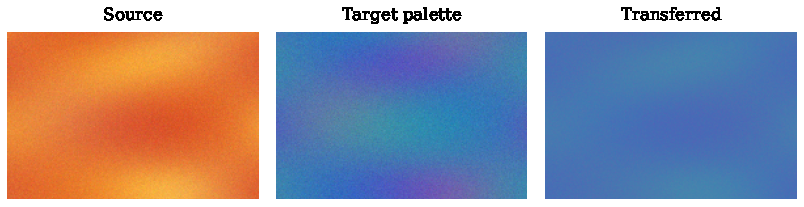
\includegraphics[width=\linewidth]{figures/fig_color_transfer.pdf}
    \caption{Image color transfer via optimal transport. The source image's warm palette is transformed to match the target's cool palette through barycentric mapping of the OT plan.}
    \label{fig:color_transfer}
\end{figure}

\begin{figure}[t]
    \centering
    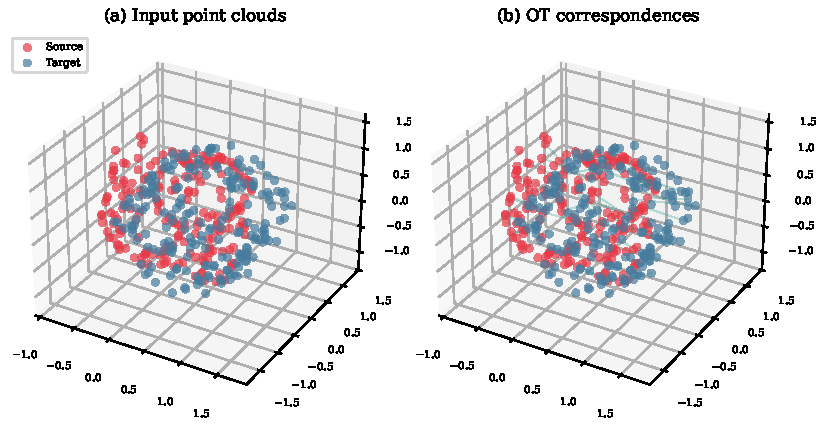
\includegraphics[width=\linewidth]{figures/fig_point_cloud.pdf}
    \caption{3D point cloud matching. (a)~Source and target point clouds. (b)~OT correspondences (green lines) connecting matched points.}
    \label{fig:point_cloud}
\end{figure}
